\documentclass{article}
\usepackage[backend=biber,natbib=true,style=alphabetic,maxbibnames=50]{biblatex}
\addbibresource{/home/nqbh/reference/bib.bib}
\usepackage[utf8]{vietnam}
\usepackage{tocloft}
\renewcommand{\cftsecleader}{\cftdotfill{\cftdotsep}}
\usepackage[colorlinks=true,linkcolor=blue,urlcolor=red,citecolor=magenta]{hyperref}
\usepackage{amsmath,amssymb,amsthm,float,graphicx,mathtools,tikz}
\usetikzlibrary{angles,calc,intersections,matrix,patterns,quotes,shadings}
\allowdisplaybreaks
\newtheorem{assumption}{Assumption}
\newtheorem{baitoan}{}
\newtheorem{cauhoi}{Câu hỏi}
\newtheorem{conjecture}{Conjecture}
\newtheorem{corollary}{Corollary}
\newtheorem{dangtoan}{Dạng toán}
\newtheorem{definition}{Definition}
\newtheorem{dinhly}{Định lý}
\newtheorem{dinhnghia}{Định nghĩa}
\newtheorem{example}{Example}
\newtheorem{ghichu}{Ghi chú}
\newtheorem{hequa}{Hệ quả}
\newtheorem{hypothesis}{Hypothesis}
\newtheorem{lemma}{Lemma}
\newtheorem{luuy}{Lưu ý}
\newtheorem{nhanxet}{Nhận xét}
\newtheorem{notation}{Notation}
\newtheorem{note}{Note}
\newtheorem{principle}{Principle}
\newtheorem{problem}{Problem}
\newtheorem{proposition}{Proposition}
\newtheorem{question}{Question}
\newtheorem{remark}{Remark}
\newtheorem{theorem}{Theorem}
\newtheorem{vidu}{Ví dụ}
\usepackage[left=1cm,right=1cm,top=5mm,bottom=5mm,footskip=4mm]{geometry}
\def\labelitemii{$\circ$}
\DeclareRobustCommand{\divby}{%
	\mathrel{\vbox{\baselineskip.65ex\lineskiplimit0pt\hbox{.}\hbox{.}\hbox{.}}}%
}
\def\labelitemii{$\circ$}

\title{Problem: Regular Triangular Pyramids {\it\&} Regular Quadrilateral Pyramids -- Bài Tập: Hình Chóp Tam Giác Đều {\it\&} Hình Chóp Tứ Giác Đều}
\author{Nguyễn Quản Bá Hồng\footnote{A Scientist {\it\&} Creative Artist Wannabe. E-mail: {\tt nguyenquanbahong@gmail.com}. Bến Tre City, Việt Nam.}}
\date{\today}

\begin{document}
\maketitle
\begin{abstract}
	This text is a part of the series {\it Some Topics in Elementary STEM \& Beyond}:
	
	{\sc url}: \url{https://nqbh.github.io/elementary_STEM}.
	
	Latest version:
	\begin{itemize}
		\item {\it Problem: Regular Triangular Pyramids {\it\&} Regular Quadrilateral Pyramids -- Bài Tập: Hình Chóp Tam Giác Đều {\it\&} Hình Chóp Tứ Giác Đều}.
		
		PDF: {\sc url}: \url{.pdf}.
		
		\TeX: {\sc url}: \url{.tex}.
		\item {\it Problem \& Solution: Regular Triangular Pyramids \& Regular Quadrilateral Pyramids -- Bài Tập \& Lời Giải: Hình Chóp Tam Giác Đều \& Hình Chóp Tứ Giác Đều}.
		
		PDF: {\sc url}: \url{.pdf}.
		
		\TeX: {\sc url}: \url{.tex}.
	\end{itemize}
\end{abstract}
\tableofcontents

%------------------------------------------------------------------------------%

\section{Regular Triangular Pyramids -- Hình Chóp Tam Giác Đều}
Hình chóp tam giác đều $S.ABC$ có 4 mặt, 6 cạnh. Mặt đáy $ABC$ là 1 tam giác đều. 3 mặt bên $SAB,SBC,SCA$ là 3 tam giác cân tại $S$. 3 cạnh đáy bằng nhau: $AB = BC = CA$. 3 cạnh bên bằng nhau: $SA = SB = SC$. $S$ gọi là \textit{đỉnh} của hình chóp tam giác đều $S.ABC$.
\begin{center}
	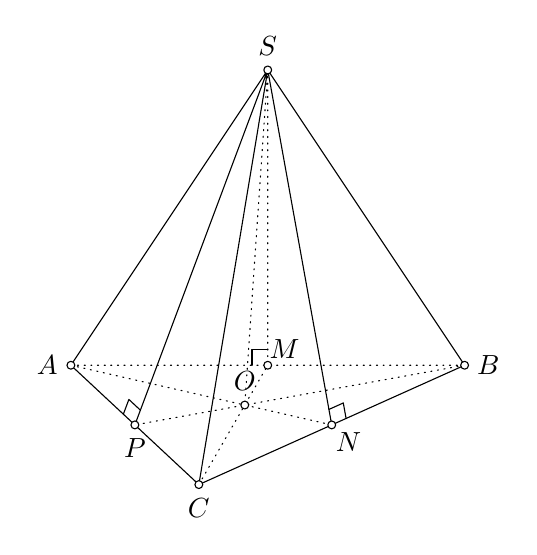
\begin{tikzpicture}[join=round,cap=round]
		\def\a{2.5}
		\pgfmathsetmacro\b{\a *cos(60) + .5}
		\path
		(180:\a) coordinate (A)
		(-120:\b) coordinate (C)
		(0:\a) coordinate (B)
		(90:1.5*\a) coordinate (S)
		($(A)!.5!(B)$) coordinate (M)
		($(B)!.5!(C)$) coordinate (N)
		($(C)!.5!(A)$) coordinate (P)
		(intersection of A--N and B--P) coordinate (O);
		\draw pic[draw,angle radius=2mm]{right angle = A--M--S};
		\draw pic[draw,angle radius=2mm]{right angle = B--N--S};
		\draw pic[draw,angle radius=2mm]{right angle = A--P--S};
		\draw[dotted] (A)--(B) (S)--(M) (A)--(N) (B)--(P) (C)--(M) (S)--(O);
		\draw (A)--(C)--(B)--(S)--cycle (S)--(C) (S)--(P) (S)--(N);
		\foreach \x in {} \draw[fill=white] (\x) circle (.05);
		\foreach \x/\g in {A/180,B/0,C/-90,S/90,M/45,N/-45,P/-90,O/90} \draw[fill=white] (\x) circle (.05) + (\g:.3) node{$\x$};
	\end{tikzpicture}
\end{center}

\subsection{Diện Tích Xung Quanh của Hình Chóp Tam Giác Đều}

\begin{dinhnghia}[Diện tích xung quanh \& trung đoạn của hình chóp tam giác đều]
	Với hình chóp tam giác đều $S.ABC$. Tổng diện tích của 3 tam giác (mặt bên) $SAB,SBC,SCA$ gọi là {\rm diện tích xung quanh} của hình chóp tam giác đều $S.ABC$: $S_{{\rm xq},S.ABC}\coloneqq S_{SAB} + S_{SBC} + S_{SCA}$. Gọi $SM,SN,SP$ lần lượt là đường cao của $\Delta SAB,SBC,SCA$. Mỗi đoạn thẳng $SM,SN,SP$ đều được gọi là {\rm trung đoạn} của hình chóp tam giác đều $S.ABC$.
\end{dinhnghia}

\begin{dinhly}
	Diện tích xung quanh của hình chóp tam giác đều bằng nửa tích của chu vi đáy với độ dài trung đoạn.
\end{dinhly}

\begin{proof}[Chứng minh]
	Vì $SA = SB = SC$ \& $AB = BC = CA$ nên $\Delta SAB = \Delta SBC = \Delta SCA$ (c.c.c) suy ra $SM = SN = SP$ (3 đường cao tương ứng). Đặt $d\coloneqq SM = SN = SP$. Có: $S_{{\rm xq},S.ABC}\coloneqq S_{SAB} + S_{SBC} + S_{SCA} = \frac{1}{2}AB\cdot SM + \frac{1}{2}BC\cdot SN + \frac{1}{2}BC\cdot SP = \frac{1}{2}d\cdot AB + \frac{1}{2}d\cdot BC + \frac{1}{2}d\cdot CA = \frac{1}{2}d(AB + BC + CA) = \frac{1}{2}dC_{ABC}$.
\end{proof}

\begin{nhanxet}
	Nhờ chứng minh này, dễ thấy định lý trên, i.e., công thức tính diện tích xung quanh $S_{\rm xq} = \frac{1}{2}Cd$ vẫn đúng với các hình chóp tam giác có 3 trung đoạn bằng nhau với đáy không nhất thiết phải là tam giác đều.
\end{nhanxet}
\noindent$\star$ {\sf Công thức tính diện tích xung quanh của hình chóp tam giác đều:} \fbox{$S_{\rm xq} = \frac{1}{2}Cd = \frac{3}{2}ad$}, trong đó $S_{\rm xq}$: \textit{diện tích xung quanh}, $C$: \textit{chu vi đáy}, $a$: \textit{độ dài cạnh} của tam giác đều mặt đáy, $C = 3a$, $d$: \textit{độ dài trung đoạn} của hình chóp tam giác đều.

\begin{baitoan}
	Cho 1 hình chóp tam giác đều có độ dài cạnh đáy bằng $a$ \& độ dài trung đoạn bằng $d$. Tính diện tích xung quanh của hình chóp tam giác đều đó.
\end{baitoan}

\begin{proof}[Giải]
	Diện tích xung quanh của hình chóp tam giác đều đó: $S_{\rm xq} = \frac{1}{2}Cd = \frac{3}{2}ad$.
\end{proof}

\begin{baitoan}
	Cho 1 hình chóp tam giác đều có độ dài cạnh đáy bằng $a$ \& diện tích xung quanh bằng $S_{\rm xq}$. Tính độ dài trung đoạn của hình chóp tam giác đều đó.
\end{baitoan}

\begin{proof}[Giải]
	Độ dài trung đoạn của hình chóp tam giác đều đó: $d = \dfrac{2S_{\rm xq}}{C} = \dfrac{2S_{\rm xq}}{3C}$.
\end{proof}

\begin{baitoan}
	Cho 1 hình chóp tam giác đều có độ dài trung đoạn bằng $d$ \& diện tích xung quanh bằng $S_{\rm xq}$. Tính chu vi đáy \& độ dài cạnh đáy của hình chóp tam giác đều đó.
\end{baitoan}

\begin{proof}[Giải]
	Chu vi đáy \& độ dài cạnh đáy của hình chóp tam giác đều đó lần lượt là: $C = \dfrac{2S_{\rm xq}}{d}$, $a = \dfrac{C}{3} = \dfrac{2S_{\rm xq}}{3d}$.
\end{proof}

\subsection{Diện Tích Toàn Phần của Hình Chóp Tam Giác Đều}
\noindent$\star$ {\sf Công thức tính diện tích toàn phần của hình chóp tam giác đều:}
\begin{align*}
	\boxed{S_{\rm tp} = S_{\rm xq} + S_{\footnotesize\mbox{\rm đ}} = \frac{1}{2}Cd + \frac{a^2\sqrt{3}}{4} = \frac{3}{2}ad + \frac{a^2\sqrt{3}}{4}.}
\end{align*}

\subsection{Thể Tích của Hình Chóp Tam Giác Đều}

\begin{dinhly}
	Thể tích của hình chóp tam giác đều bằng $\frac{1}{3}$ tích của diện tích đáy với chiều cao.
\end{dinhly}
\noindent$\star$ {\sf Công thức tính thể tích của hình chóp tam giác đều:} \fbox{$V = \dfrac{1}{3}S_{\footnotesize\mbox{\rm đ}}h = \dfrac{a^2h\sqrt{3}}{12}$}, trong đó $V$: \textit{thể tích}, $S_{\footnotesize\mbox{\rm đ}}$: \textit{diện tích đáy}, $h$: \textit{chiều cao} của hình chóp tam giác đều.

%------------------------------------------------------------------------------%

\section{Regular Quadrilateral Pyramids -- Hình Chóp Tứ Giác Đều}

%------------------------------------------------------------------------------%

\section{Miscellaneous}

%------------------------------------------------------------------------------%

\printbibliography[heading=bibintoc]
	
\end{document}